\documentclass[shortAfour,sageh.bst]{sagej}

\usepackage{moreverb,url,natbib, multirow, tabularx}
\usepackage[colorlinks,bookmarksopen,bookmarksnumbered,citecolor=red,urlcolor=red]{hyperref}



\usepackage{natbib}

\usepackage{bm}
     \def\Var{{\rm Var}\,}
     \def\Cov{{\rm Cov}\,}
     \def\mean{{\rm mean}\,}
     \def\E{{\rm E}\,}
  	 \def\Corr{{\rm Corr}\,}

\usepackage{xcolor}

\renewcommand{\appendixname}{Supplementary Material}

\usepackage{hyperref}
\usepackage{rotating}
\usepackage{booktabs}
\usepackage{makecell}
\usepackage{dcolumn}
\newcolumntype{d}[1]{D{.}{.}{#1}}
\usepackage{booktabs}
\usepackage{longtable}
\usepackage{array}
\usepackage{multirow}
\usepackage{wrapfig}
\usepackage{float}
\usepackage{colortbl}
\usepackage{pdflscape}
\usepackage{tabu}
\usepackage{threeparttable}
\usepackage{threeparttablex}
\usepackage[normalem]{ulem}
\usepackage{makecell}
\usepackage{xcolor}


\begin{document}

\title{Modeling the impacts of park access on health outcomes: a utility-based
accessibility approach}

\runninghead{Macfarlane \emph{et al}.}

\author{Gregory S. Macfarlane\affilnum{1}, Nico Boyd\affilnum{2}, John E. Taylor\affilnum{3}, Kari Watkins\affilnum{3}}

\affiliation{\affilnum{}{}\\\affilnum{}{}\\\affilnum{}{}}

\corrauth{Gregory Macfarlane, 430 Engineering Building, Provo UT 84663}

\email{\href{mailto:gregmacfarlane@byu.edu}{\nolinkurl{gregmacfarlane@byu.edu}}}

\begin{abstract}
Recent research has underscored the potential for public green spaces to
influence individual and societal health outcomes, but empirical
measurements of such influences have yielded mixed results to date, with
particular disagreement surrounding how access to parks ought to be
defined while controlling for alternate explanations. In this paper we
apply a comprehensive measure of park accessibility drawn from random
utility choice theory, which avoids arbitrary assertions of proximity
while incorporating potentially numerous amenities and attributes of
both the parks and the population. We apply this utility-based
accessibility measure to correlate Census tract-level obesity and
physical activity rate estimates from the Centers for Disease Control
and Prevention's 500 Cities project with tract-level American Community
Survey socioeconomic data in New York City, paired with geographic open
space data from New York City. Controlling for the socioeconomic
variables and spatially correlated error terms, we show a positive and
significant relationship between park access and physical activity
rates. The data also suggest a negative relationship between park access
and obesity rates, beyond what is expected through physical activity and
socioeconomics. In doing so, this research contributes a more
comprehensive modeling approach for measuring the impact of park access
on health, and may improve our understanding of the role parks and
access to them can serve in furthering public health objectives.
\end{abstract}

\keywords{Accessibility; Green Space}

\maketitle

\hypertarget{introduction}{%
\section{Introduction}\label{introduction}}

The United States and other developed nations face an epidemic of
obesity and chronic diseases, including cardiovascular diseases, chronic
respiratory diseases, diabetes, stroke, joint and bone diseases, and
cancer. These diseases can severely limit the lifespan of affected
individuals \citep{WHO2014}, with substantial financial costs for
treatment borne both privately and socially \citep{Finkelstein2009}.
Though a moderate amount of regular physical activity has been
established as an effective strategy for reducing and managing obesity
and many of the aforementioned chronic diseases
\citep{CDC2009, Durstine2013}, a large portion of U.S. adults do not
participate in sufficient physical activity \citep{Wolf2008}.

Historically, most large-scale health promotion efforts focused on
individual-level interventions intended to educate people about healthy
lifestyles and behaviors, touching on topics including diet and
exercise. Over the last several years a new \emph{social} model of
health has evolved, described by \citet{Duhl1999} ``as an outcome of the
effects of socioeconomic status, culture, environmental conditions,
housing, employment and community
influences''\citeyearpar[p.7]{Duhl1999}. In this new paradigm, resources
provided via civil infrastructure --- in particular parks and other
public green spaces --- play a crucial role in promoting and sustaining
public health \citep{Bedimo-Rung2005, Wells2007, Coutts2008}. After all,
it does little to educate individuals on the importance of exercise if
their community is designed and built in such a way that such exercise
is expensive, unenjoyable, or unsafe. It is similarly necessary for
urban planners to identify which neighborhoods have access to quality
green space, and which neighborhoods need intervention in the form of
new or rehabilitated green space, or improved transportation access to
existing quality green space.

But in spite of the potential for green spaces to influence public
health outcomes and numerous studies attempting to empirically estimate
the strength of these outcomes, evidence to date has been mixed. A major
challenge researchers have faced is a proliferation of techniques for
measuring access to green spaces, of which many are plausible but lack
robust theoretical bases.

In this paper, we apply a holistic and flexible measurement for park
accessibility based in activity location choice theory. This
utility-based accessibility measure compares the continuous distance to
all parks in the region, weighted against the sizes of each park and its
other assorted amenities. We apply this measure to study the link
between park accessibility and attractiveness and census tract-level
aggregate physical activity participation and obesity rates in New York
City, controlling for spatially correlated unobserved effects, spatial
spillovers of covariates, and tract-level socioeconomic characteristics.
We also demonstrate how the utility-based accessibility metric can
potentially be expanded to account for other measures of a park's
attractiveness in the form of various park amenities. The paper
concludes with a discussion of opportunities for future research.

\hypertarget{literature-review}{%
\section{Literature Review}\label{literature-review}}

\label{sec:litreview} The question of how green space in the urban
environment affects the physical, emotional, and mental well-being of
urban residents is not new to the academic literature. Comprehensive
reviews and analysis of this literature up to 2007 can be had from
\citet{tzoulas2007promoting}, and for the subsequent decade from
\citet{kabisch2015human}. In spite of the depth of this research arena
--- or perhaps because of it --- quantitative approaches for assessing
both health outcomes and access to green space vary widely. It is
therefore not surprising that in a meta-analysis of 20 recent peer
reviewed journal articles exploring the relationship between access to
parks and objectively measured physical activity, \citet{Bancroft2015}
found that five studies reported a significant positive association, six
studies produced mixed results, and nine studies found no association at
all.

Loosely defined, the \emph{accessibility} of an arbitrary place
describes the ease with which people can accomplish activities there.
Accessibility is an abstract concept with tempting quantifiability
\citep{Handy1997}, but objective quantification may not be strictly
necessary. For example, \citet{takano2002urban} showed improved survival
rates among senior citizens in Japan who self-reported having access to
qualitatively good walking spaces. Though encouraging, this result could
simply reveal self-selection: Those seniors who felt the walking space
was good were those who chose to enjoy it. Urban planners seeking to
evaluate which residents have good access to quality green space may
desire objective and therefore comparable measures.

\citet{Dong2006} present a helpful mathematical hierarchy of common
quantitative mechanisms for calculating access, which we follow here.
Consider a person residing at point \(i\) in a city with parks
\(j \in 1 \ldots J\). An analyst might consider point \(i\) as ``having
access'' to a park if the distance to the park \(d_{ij}\) is within an
``isochrone,'' or a geometric buffer defined by some threshold \(D\),

\begin{equation}\label{eq:isochrone}
A_i = \begin{cases} 
      1 & d_{ij}\leq D\\
      0 & d_{ij} > D
   \end{cases}
\end{equation}

Applications of this isochrone-based framework are easily derived and
relatively common. ParkScore \citep{parkscore2019} is a sophisticated
application of this approach where \(D\) is a carefully calculated
10-minute network-bound walk, paired with a demographic analysis of
areas within and outside of this threshold. \citet{devries2003natural}
showed the amount of green space within a 3-kilometer radius was
positively associated with a suite of self-reported health outcomes.
Similarly, \citet{devries2013streetscape} showed that streetscape
greenery within 500 meters of a residence was associated with perceived
general health. Conversely, \citet{carlson2012interactions} found no
relationship between the health of senior citizens and the number of
parks within 500 meters.

Another common access measure fits in this category, where
distance-based isochrones are replaced with political, geographical, or
statistical boundaries. For example, \citet{Mitchell2008} find that
inequalities in health outcomes attributable to income are mitigated in
statistical areas with a greater percentage of green space. These are
especially common in comparative macroscopic studies, such as the
positive relationships found by \citet{West2012} between density of park
land in a metropolitan area and self-reported population health
indicators derived from the Behavioral Risk Factor Surveillance System
(BRFSS). On the other hand, \citet{Larson2016} found no relationship
between physical health and park quantity, quality, and accessibility in
44 U.S. cities and self-reported scores on the Gallup-Healthways
Wellbeing Index. At the sub-metropolitan level, \citet{Stark2014} found
a significant relationship in New York City between the percent of a
residential ZIP code that is park space and objectively measured body
mass index (BMI). It is also possible to attenuate an isochrone with
various factors; for instance, \citet{Dias2019} considered road safety
perception as an extenuating factor in the effective distance to a park.

In spite of the flexibility of adapted isochrone techniques, the
arbitrary definitions necessarily imposed by researchers in its
application can inhibit holistic analysis \citep{Logan2017}. A somewhat
more complete approach is the so-called ``gravity'' accessibility
statistic. In this case the accessibility of point \(i\) is the
denominator of the gravity formulation of a trip distribution model,
\begin{equation}\label{eq:gravity}
A_i = \sum_{j = 1}^J S_j f(d_{ij})
\end{equation} where \(S_j\) is the ``size'' of each park literally
(i.e.~acres) or abstractly (i.e. trip attractions) and \(f(d_{ij})\) is
a monotonically decreasing cost function, usually a negative
exponential. \citet{Dong2006} note that the isochrone framework is a
special case of the gravity model where \(f(d_{ij})\) is a binary
function and \(S_j = 1\). \citet{Giles-Corti2005} compare various
gravity-based accessibility scores with an isochrone specification and
show that the former are more predictive of walking behavior; that is,
the attributes of a park influence walking more than merely the distance
to it. \citet{hillsdon2006relationship} found no relationship between a
gravity-based accessibility term and self-reported physical activity
among middle-aged individuals in Norwich, England. \citet{Zhang2011}
developed a population-weighted, gravity-based accessibility to parks
metric with a national scope, though they do not examine its correlation
with health outcomes.

A third accessibility mechanism is a utility-based specification, termed
as such for being derived from random utility choice theory. Consider
that an individual living at point \(i\) is choosing a park for a
recreation activity. If we apply the multinomial logit model
\citep{McFadden1974}, the expected consumer surplus enjoyed by this
individual can be shown to be \begin{equation}\label{eq:utility}
A_i = \ln\left({\sum_{j = 1}^J\exp(V_{ij})}\right) + C
\end{equation} where parks are differentiated from each other by their
relative measurable \emph{utilities}, \(V_{ij}\). \(C\) is an unknown
constant, but the difference in consumer surplus between two points
\(i\) and \(k\) can be quantitatively compared as \(A_i - A_k\)
\citep{Bruce1977}. In principle, \(V\) may include any measurable
attributes of either the choice maker or the park, and is typically
represented as a linear-in-parameters function of destination attributes
\(X_j\) and the travel cost \(d_{ij}\),
\begin{equation}\label{eq:utilityV}
V_{ij} = X_j\boldsymbol{\beta} + \beta_d * d_{ij}
\end{equation} The coefficients \(\boldsymbol{\beta}\) are frequently
estimated from household surveys, though in the absence of a survey we
may assert reasonable values.

Note that the gravity formulation is itself a special case of the
utility-based specification where
\(\exp(X_j\boldsymbol{\beta} + \beta_d d_{ij}) = X_j f(d_{ij})\)
\citep{Daly1982}. The distinction between gravity and utility-based
specification is meaningful, however. Primarily, it becomes possible to
construct accessibility statistics based on revealed behavioral
preferences rather than calibrated or asserted values \citep{Handy1997}.
\citet{Kinnell2006} collected a choice-based survey sufficient to
construct a utility-based measure, though they do not do so. Similarly,
\citet{Kaczynski2016} present what is effectively a utility-based score
called ``ParkIndex'', with the explicit motivation of developing a
uniformly applicable park accessibility statistic, though they limit
this statistic as a way to add heterogeneity within an isochrone
analysis.

Both gravity and utility-based specifications hold several advantages
relative to isochrone-based accessibility metrics more commonly found in
the literature. First, all individuals are defined as having some access
to all parks, rather than an arbitrary cutoff asserted by the
researcher. This allows for the fact that some people are more or less
sensitive to distances, and that distance is a continuous, non-binary
phenomenon. It defies reason to assume a person living 11 minutes via
walking from a park always has meaningfully different accessibility than
someone living 9 minutes away. Second, the random utility formulation
allows the researcher to include -- in principle -- any attribute of the
park as part of its utility specification. This suggests that not all
parks are equal, and that a large park with many amenities such as
Central Park in Manhattan may provide health and activity benefits over
a much larger area than a smaller community square.

In spite of its flexibility and basis in choice theory, utility-based
accessibility measures have not received much application in the park
accessibility literature compared with distance-based or even
gravity-based measures. \citet{Vale2016} present a descriptive
classification of active accessibility techniques, and explicitly
dismiss utility-based metrics for incorporating randomness. This is a
curious decision: The accessibility formula presented in Equation
\ref{eq:utility} is the expectation of a random utility process, but the
measure is not in and of itself random any more than the gravity model
is random. Utility-based accessibility metrics are commonly used,
however, in alternatives analyses of transit infrastructure improvements
\citep{DeJong2007}. A reason for this is likely that a regional travel
demand model is available to the analysts, thus making calibrated and
multimodal logsums readily available \citep{Geurs2010}.

To our knowledge, there has been no previous attempt to examine access
to parks in a metropolitan area using a utility-based definition as the
primary indicator of access. Consequently, there has also been no
previous effort to examine the effect of park access on health outcomes
using this theoretically attractive technique. In this study, we first
develop a utility-based measure of park access in New York City, and
then apply this measure to study the effect of access to public parks on
aggregate health outcomes.

\hypertarget{empirical-application}{%
\section{Empirical Application}\label{empirical-application}}

In this section, we develop a model with data for New York City, where
we compute a set of utility-based accessibility to parks scores for each
tract and model the relationship between this measure and physical
activity rates, controlling for spatial effects and socioeconomic
factors. We subsequently model the effect of the accessibility metric on
obesity rates, accounting for physical activity and the other controls.

\hypertarget{data}{%
\subsection{Data}\label{data}}

This study uses data available to the public from a variety of federal
and state data agencies\footnote{The datasets, as well as the analysis
  code, are available on GitHub at
  \url{https://github.com/gregmacfarlane/parks_access}.}. The Centers
for Disease Control and Prevention makes small-area estimates on key
health indicators available through its 500 Cities data program
\citep{CDC5002016}. The indicators are multilevel aggregations and
imputations of BRFSS responses \citep{Wang2018, Wang2017}, and have been
recently used to study the tract-level link between gentrification and
urban health \citep{Gibbons2018}. We use two indicators as our dependent
variables in this study: the share of adults in a Census tract who are
obese, and the share of adults who participate in no leisure-time
physical activity. To improve clarity in our interpretation, we use the
complement of the second variable --- the share of tract adults who
participate in \emph{some} physical activity --- even if the amount may
not be sufficient to affect overall health. Both indicators are obtained
for the year 2016.

To the health data, we join socioeconomic data collected through the
Census Bureau API via the \texttt{tidycensus} package for R
\citep{Walker2019}. The primary dataset is a geographic polygons layer
of Census tracts in the five boroughs of New York City. We append to
each Census tract relevant socioeconomic data for each tract from the
American Community Survey 2013-2017 5-year estimates. For a small
handful of tracts in our sample, Census supressed the median income
estimate; these appear to be primarily wealthy tracts and in almost all
cases the CDC estimates of obesity and physical activity are missing as
well. After removing these tracts from the estimation dataset, we have
2,102 complete cases. Table \ref{tab:tractsdata} presents key
descriptive statistics for these data.

In a destination choice framework, the tracts represent the ``origins''
and the ``destinations'' are parks and green spaces in New York City. We
retrieved a polygons layer of public parks and green spaces within New
York City's municipal boundaries and checked it for accuracy and
relevance \citep{nycparks}. Upon inspection, we removed several
facilities that do not qualify as publicly accessible green space, such
as Yankee Stadium, Citi Field, and their surrounding parking lots. We
also removed parks of less than half an acre in size, as these appear to
be predominantly planted medians rather than legitimate public green
space. We consolidated individual geographic polygons comprising a
single facility --- as is the case in Flushing Meadows --- and
eliminated sub-facilities such as tennis courts or baseball fields
included within larger park facilities. Instead of these distinct
sub-facilities, we created variables for each containing park indicating
the presence of sports courts, playgrounds, and trails. These operations
leave us with 1,191 distinct green spaces; For each park, we calculate
the size of the park in acres.

\begin{table*}

\caption{\label{tab:tractsdata}Descriptive Statistics of Tract and Park Variables}
\centering
\resizebox{\linewidth}{!}{
\begin{tabular}[t]{l>{\raggedright\arraybackslash}p{2in}rlrl}
\toprule
  & Description & Minimum & Median (IQR) & Maximum & Source\\
\midrule
\addlinespace[0.3em]
\multicolumn{6}{l}{\textbf{Tract Variables, N = 2102}}\\
\hspace{1em}Obesity & Share of adults over 18 who are obese & 9.60 & \makecell{24.50\\ (19.60, 30.50)} & 44.20 & CDC 500 Cities\\
\hspace{1em}Physical Activity & Share of adults over 18 who engage in some leisure-time physical activity & 48.10 & \makecell{69.50\\ (64.70, 74.60)} & 89.10 & CDC 500 Cities\\
\hspace{1em}Income & Median tract income & 9053.00 & \makecell{59,592.50\\ (41,928.25, 79,092.75)} & 250001.00 & ACS\\
\hspace{1em}Density & Households per square kilometer & 9.20 & \makecell{5,848.46\\ (3,173.62, 9,674.36)} & 43621.52 & ACS\\
\hspace{1em}Fulltime & Share of adults over 18 with full-time work & 8.80 & \makecell{49.48\\ (44.45, 55.29)} & 100.00 & ACS\\
\hspace{1em}College & Share of adults over 24 with a college degree & 0.61 & \makecell{16.30\\ (12.37, 20.11)} & 44.94 & ACS\\
\hspace{1em}Single & Share of adults over 18 living alone or in a non-partnership household & 16.38 & \makecell{59.39\\ (50.30, 68.65)} & 100.00 & ACS\\
\hspace{1em}Youth & Share of population under 18 & 0.00 & \makecell{20.54\\ (16.79, 24.92)} & 64.07 & ACS\\
\hspace{1em}Young adults & Share of population between 18 and 34 & 0.00 & \makecell{25.73\\ (21.66, 29.98)} & 86.75 & ACS\\
\hspace{1em}Seniors & Share of population who are 65 and over & 0.00 & \makecell{12.83\\ (9.47, 16.88)} & 89.88 & ACS\\
\hspace{1em}Black & Share of population who is black & 0.00 & \makecell{10.03\\ (2.13, 44.62)} & 220.65 & ACS\\
\hspace{1em}Asian & Share of population who is Asian & 0.00 & \makecell{7.66\\ (2.40, 20.78)} & 88.07 & ACS\\
\hspace{1em}Hispanic & Share of population who is Hispanic & 0.00 & \makecell{19.07\\ (9.39, 41.07)} & 96.27 & ACS\\
\hspace{1em}Other & Share of population who belong to other minority groups & 0.00 & \makecell{0.00\\ (0.00, 0.53)} & 19.47 & ACS\\
\addlinespace[0.3em]
\multicolumn{6}{l}{\textbf{Park Variables, N = 1191}}\\
\hspace{1em}Size & Park size in acres & 0.50 & \makecell{1.57\\ (0.94, 4.45)} & 1961.00 & NYC\\
\hspace{1em}Courts & Presence of sport courts / ball fields & 0.00 & \makecell{0.00\\ (0.00, 0.00)} & 1.00 & NYC\\
\hspace{1em}Playgrounds & Presence of playgrounds & 0.00 & \makecell{0.00\\ (0.00, 1.00)} & 1.00 & NYC\\
\hspace{1em}Trails & Presence of trails & 0.00 & \makecell{0.00\\ (0.00, 0.00)} & 1.00 & NYC\\
\bottomrule
\end{tabular}}
\end{table*}

\hypertarget{accessibility}{%
\subsection{Accessibility}\label{accessibility}}

\label{subsec:accessibility}

We calculate a pair of utility-based accessibility statistics for each
tract in New York City. The most basic utility specification includes
only the park size in acres and the Euclidean distance from the
population-weighted tract centroid to the nearest boundary of the park
in miles, \begin{equation}\label{eq:u_access}
V_{ij} = \lambda_s * \log(size_j) + \lambda_d * \log(distance_{ij})
\end{equation} There are a few cases where the population-weighted tract
centroid lies on or within the boundary of a park; for these cases we
assert that the minimum possible distance is one tenth of a mile. The
logarithmic transform allows for diminishing marginal utility of
distance and park size: A 1-mile increase to a trip matters more for a
1-mile trip than a 10-mile trip. \citet{Macfarlane2019} estimated
destination choice parameters for park trips in Alameda County
(Oakland), California by applying this utility specification to
passively collected mobile device data, obtaining values of
\(\lambda_s = 0.373\) and \(\lambda_d = -1.76\). The ratio of these
estimates implies people are willing to travel roughly six times further
to reach a park twice as large. We do not have access to the necessary
data to repeat the \citet{Macfarlane2019} methodology in New York, and
the public parks datasets in Alameda County are not sufficiently
detailed to perform the present accessibility analysis there. In the
absence of park trip destination choice coefficients in New York City,
we adopt these previous estimates.

\citet{Kinnell2006} surveyed park users in New Jersey and applied a
multinomial logit model to determine which factors influence a park's
perceived utility as a park trip destination. By transferring estimates
of common variables between our data and this survey-based model, we can
create a second utility specification as
\begin{equation}\label{eq:u_multi}
\begin{split}
V_{ij} & = \lambda_s * \log(size_j) + \lambda_d * \log(distance_{ij}) + \\ 
  & \quad \lambda_t * trails + \lambda_{c} * courts + \lambda_p * playgrounds
\end{split}
\end{equation} with \(\lambda_t = 0.99\), \(\lambda_c = 0.43\), and
\(\lambda_p = 0.26\). Kinnell et al.~did not transform their size and
distance estimates, so we retain the previously estimated and applied
values. We assume that the other covariates in the model which we do not
have available to us (e.g., boat launches, picnic areas) are orthogonal
to the included parameters and leaving them out will not affect the
values of the included coefficients.

We then calculate the utility-based accessibility of each tract \(A_i\)
as defined in Equation \ref{eq:utility} under each utility
specification. Recall that the total value of the accessibility is
relative to an unknown scalar \(C\); for this reason we standardize the
accessibility values for all tracts within each utility specification,
\begin{equation}\label{eq:v_logged}
A_i' = \frac{A_i - \bar{\boldsymbol{A}}}
            {\sigma_{\boldsymbol{A}}}
\end{equation}

Figure \ref{fig:map} shows a map of New York City with each tract
highlighted based on its relative size and distance utility-based
accessibility score (Equation \ref{eq:u_access}). The most continuous
region of good park access is in upper Manhattan and the Bronx,
bracketed by Central Park and the Bronx River. Conversely, some of the
poorest-accessibility areas are in Brooklyn tracts not immediately
adjacent to Prospect Park. Because the accessibility statistic is
normalized, the worst values are slightly below \(-3\), the best
somewhere above \(3\).

For comparative purposes, we also employ an isochrone analysis using the
10-minute walk threshold calculated for ParkScore \citep{parkscore2019}.
If the population-weighted centroid of a tract is within a 10-minute
walk of a green space as defined by ParkScore, the tract is considered
as having ``access'' to a park. The centroid is necessary as all tracts
in New York City have at least \emph{some} intersection with the
10-minute walk buffer; as it is, only 24 of the 2,102 tract centroids
are not located within this buffer.

\begin{figure*}
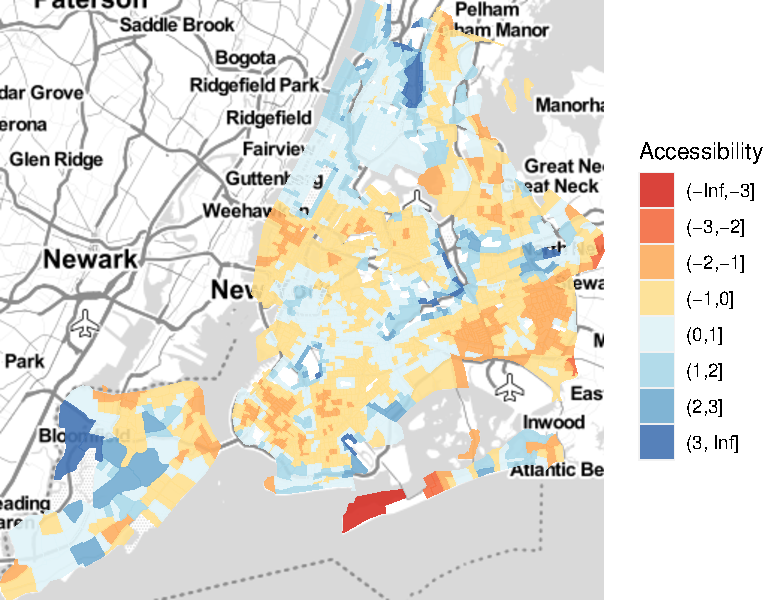
\includegraphics{manuscript_files/figure-latex/map-1} \caption{Normalized utility-based park accessibility values in New York City.}\label{fig:map}
\end{figure*}

\hypertarget{model}{%
\subsection{Model}\label{model}}

\label{subsec:model}

We predict either the physical activity or the obesity rate (\(y\)) in a
census tract as a linear function of the tract's sociodemographic
characteristics \(X\) and accessibility to parks \(\boldsymbol{A}\),
\begin{equation}\label{eq:themodel}
 \boldsymbol{y} = X\boldsymbol{\beta} + \beta_{a}\boldsymbol{A} + \boldsymbol{\varepsilon}
\end{equation} where \(X\) is a matrix of dimension \(n\times p\) where
\(n\) is the number of observations and \(p\) is the number of predictor
variables, and \(\boldsymbol{\beta}\) is a \(p\times 1\) vector of
estimated parameters. The accessibility vector \(\boldsymbol{A}\)
influences physical activity or obesity rates by the single estimated
parameter \(\beta_a\), and a vector \(\boldsymbol{\varepsilon}\)
represents the model residual as a random variable.

As the observations are related to each other spatially, it is likely
that this process involves spatial spillovers of one kind or another. A
complete treatment of spatial econometrics is not warranted here; the
reader is directed to \citet{LeSage2009} as well as \citet{LeSage2014}.
Suffice it to say that the presence of spatial data generating processes
can negatively affect econometric interpretation in a variety of ways.
Each of these processes rely on spatial autoregression, where elements
of some random variable \(x\) are spatially dependent on other elements,
\begin{equation}\label{eq:autoregression}
 \boldsymbol{x} = \rho W \boldsymbol{x} + \boldsymbol{\varepsilon}
\end{equation} with the strength of dependence an estimated parameter
\(\rho\), the structure of spatial dependence governed by the asserted
matrix \(W\) (details of \(W\) follow below), and some random
uncorrelated residual \(\varepsilon\). A collection of models is
available to represent spatial autodependence in the model residuals,
the independent variables, and the dependent variable.

The specific spatial model applied is both an econometric choice --- as
improperly specified spatial models can lead to inconsistent estimates
of model parameters and standard errors --- as well as a philosophical
choice about the likely structure of spillovers in the problem at hand.
In case of physical activity and obesity rates, we believe that the
outcomes are locally dependent: That is, a particular individual decides
whether or not to participate in physical activity independently of
whether his or her neighbors participate in physical activity. This does
not mean that we think it impossible that the socioeconomic variables of
neighboring tracts do not play a role. Mathematically, we assert that
the autodependence relationship on the dependent variable
\(\boldsymbol{y} = \rho W \boldsymbol{y} + \ldots\) has \(\rho = 0\) in
the current case.

With this relationship ruled out, it remains a possibility that the
model residuals are spatially dependent, \begin{equation}\label{eq:SEM}
 \boldsymbol{y} = X\boldsymbol{\beta} + \beta_a \boldsymbol{A} + \boldsymbol{u}; \boldsymbol{u} = \lambda W \boldsymbol{u} + \boldsymbol{\varepsilon}
\end{equation} that the outcome is partially dependent on the
socioeconomic variables in \emph{neighboring} tracts,
\begin{equation}\label{eq:SLX}
 \boldsymbol{y} = X\boldsymbol{\beta} + \beta_a \boldsymbol{A} + W X \boldsymbol{\gamma} + \boldsymbol{\varepsilon}
\end{equation} or a linear combination of both.
\begin{equation}\label{eq:SDEM}
 \boldsymbol{y} = X\boldsymbol{\beta} + \beta_a \boldsymbol{A} + W X \boldsymbol{\gamma} + \boldsymbol{u}; \boldsymbol{u} = \lambda W \boldsymbol{u} + \boldsymbol{\varepsilon}
\end{equation} These models are referred as the spatial error model
(SEM), the spatial lag of \(X\) model (SLX), and the spatial Durbin
error model (SDEM). \citet{Pace2008} suggest that a Hausman-style test
of the estimates of \(\boldsymbol{\beta}\) derived from the OLS
(Equation \ref{eq:themodel}) and SEM (Equation \ref{eq:SEM}) can
identify whether the estimates are consistent. If the
\(\boldsymbol{\beta}\) estimates are dissimilar, both specifications are
inappropriate as they contain untreated omitted variables. Similarly, if
the SLX and SDEM estimates are dissimilar it is an indication of missing
variables in that specification. On the other hand if the estimates of
both pairs of models are similar and the residual correlation parameter
\(\lambda\) is non-zero, the model accounting for spatially dependent
residuals will produce proper estimates of the model standard errors.

Note that in the lag-\(X\) specifications (SLX and SDEM) we exclude the
accessibility component \(\boldsymbol{A}\), that is we do \emph{not}
consider that the accessibility in a neighboring zone will have an
effect on physical activity or obesity rates. In a practical sense, this
is because the accessibility term \(\boldsymbol{A}\) is itself spatially
determined.

\hypertarget{spatial-weights}{%
\subsubsection{Spatial Weights}\label{spatial-weights}}

The spatial weights matrix \(W\) is constructed of individual elements
where \(w_{ij} = 0\) if observations \(i\) and \(j\) are spatially
independent of each other, and \(w_{ij} > 0\) if \(i\) and \(j\) are
spatially related in some way. \citet{Dubin1998} presents details on
constructing \(W\), but in this study we assume that tracts sharing at
least one common border point are neighbors of each other\footnote{We
  also considered a distance-discounted weights matrix, which produced
  similar results. This matrix is selected for simplicity.}. The
elements of \(W\) are then row-standardized so that each observation has
an equal total influence from all its neighbors.

\hypertarget{results}{%
\subsection{Results}\label{results}}

To determine which spatial effects specification was appropriate, we
estimated SLX and SDEM models of physical activity participation rates
as a function of tract covariates and accessibility. These two models
are presented in Table \ref{tab:slx-sdem}. With only a few exceptions,
the SLX and SDEM coefficient estimates for corresponding covariates lie
within the 95\% confidence intervals of the other model. A Hausman-style
test \citep{Pace2008} on the coefficients assumes a null hypothesis that
the coefficients are equivalent; this test produces \(p\)-value of only
\(1.318e-23\). Though this statistic is well beneath a common hypothesis
test threshold of \(\alpha = 0.05\), we elect to retain the null
hypothesis that the coefficients are equivalent, as the differences are
at no point practically different from each other. The consequences of
rejecting the null hypothesis in this case would be to suggest a model
with spatial dependence of the dependent variable; as stated above, we
feel that such a relationship is unreasonable. As a consequence of these
analyses, we adopt the SDEM specification moving forward as the spatial
lag of the errors is significant and the overall log likelihood of the
SDEM is higher than the SLX specification.

\begin{table*}
\caption{Comparison of SLX and SDEM Coefficients}
\label{tab:slx-sdem}
\begin{tabular}{l d{2.4} d{2.4} d{2.4} c d{2.4} d{2.4} d{2.4} }
\toprule
 & \multicolumn{3}{c}{SLX} & & \multicolumn{3}{c}{SDEM} \\
\cmidrule{2-4}\cmidrule{6-8}
 & \multicolumn{1}{c}{Estimate} & \multicolumn{2}{c}{95\% Conf.Int.} & 
 & \multicolumn{1}{c}{Estimate} & \multicolumn{2}{c}{95\% Conf.Int.}\\
\midrule
% latex table generated in R 4.0.0 by xtable 1.8-4 package
% Thu Sep 24 13:27:59 2020
 (Intercept) & -15.8791 & -26.8066 & -4.9515 &   & -24.7352 & -41.5391 & -7.9312 \\ 
  log(Density) & 0.0502 & -0.1280 & 0.2284 &   & 0.1760 & 0.0371 & 0.3150 \\ 
  log(Income) & 5.8667 & 5.3476 & 6.3859 &   & 6.0134 & 5.5901 & 6.4368 \\ 
  Fulltime & 0.1157 & 0.0944 & 0.1369 &   & 0.1271 & 0.1086 & 0.1455 \\ 
  College-educated & 0.0029 & -0.0253 & 0.0311 &   & 0.0077 & -0.0156 & 0.0310 \\ 
  Single Adults & -0.0435 & -0.0623 & -0.0247 &   & -0.0365 & -0.0528 & -0.0201 \\ 
  Youth (0-17) & -0.1528 & -0.1844 & -0.1211 &   & -0.1320 & -0.1585 & -0.1055 \\ 
  Young adults (18-34) & 0.0245 & -0.0001 & 0.0492 &   & 0.0292 & 0.0092 & 0.0493 \\ 
  Seniors (65+) & 0.0108 & -0.0212 & 0.0427 &   & 0.0386 & 0.0112 & 0.0659 \\ 
  Black population share & -0.0471 & -0.0589 & -0.0353 &   & -0.0499 & -0.0586 & -0.0412 \\ 
  Asian population share & -0.0684 & -0.0828 & -0.0540 &   & -0.0764 & -0.0870 & -0.0659 \\ 
  Hispanic population share & -0.1003 & -0.1126 & -0.0881 &   & -0.1023 & -0.1114 & -0.0932 \\ 
  Other Minorities & 0.0341 & -0.0661 & 0.1343 &   & 0.0047 & -0.0837 & 0.0931 \\ 
  $\gamma$: log(Density) & 1.2513 & 0.9367 & 1.5659 &   & 1.0873 & 0.7062 & 1.4684 \\ 
  $\gamma$: log(Income) & 2.3641 & 1.5266 & 3.2016 &   & 1.9780 & 0.9563 & 2.9997 \\ 
  $\gamma$: Fulltime & -0.1346 & -0.1749 & -0.0943 &   & -0.0411 & -0.0882 & 0.0059 \\ 
  $\gamma$: College-educated & -0.1201 & -0.1692 & -0.0711 &   & -0.0704 & -0.1296 & -0.0112 \\ 
  $\gamma$: Single Adults & -0.0520 & -0.0857 & -0.0183 &   & -0.0094 & -0.0514 & 0.0325 \\ 
  $\gamma$: Youth (0-17) & -0.1013 & -0.1594 & -0.0432 &   & -0.0128 & -0.0815 & 0.0559 \\ 
  $\gamma$: Young adults (18-34) & 0.1131 & 0.0706 & 0.1555 &   & 0.0838 & 0.0334 & 0.1342 \\ 
  $\gamma$: Seniors (65+) & 0.0015 & -0.0568 & 0.0598 &   & 0.0545 & -0.0145 & 0.1235 \\ 
  $\gamma$: Black population share & 0.0099 & -0.0051 & 0.0248 &   & 0.0011 & -0.0149 & 0.0172 \\ 
  $\gamma$: Asian population share & -0.0644 & -0.0821 & -0.0467 &   & -0.0397 & -0.0582 & -0.0212 \\ 
  $\gamma$: Hispanic population share & -0.0074 & -0.0229 & 0.0081 &   & -0.0015 & -0.0185 & 0.0156 \\ 
  $\gamma$: Other Minorities & 0.1629 & -0.0725 & 0.3983 &   & 0.0723 & -0.1840 & 0.3286 \\ 
  Accessibility & 0.6575 & 0.5348 & 0.7801 &   & 0.2306 & 0.0907 & 0.3705 \\ 
  $\lambda$: spatial correlation &  &  &  &   & 0.6854 & 0.6459 & 0.7249 \\ 
  
\midrule
Log Likelihood & \multicolumn{3}{c}{$-4,815$} & & \multicolumn{3}{c}{$-4,433$}\\
Num.Obs.       & \multicolumn{3}{c}{$2,099$}   & & \multicolumn{3}{c}{$2,099$}\\
\bottomrule
\end{tabular}
\end{table*}

The coefficients in the SDEM model are of two general types: the direct
effect resulting from a tract's own attributes and the indirect effect
(\(\boldsymbol{\gamma}\)) resulting from the spatially-weighted
attributes of its neighbors. For example, a percentage point increase in
the share of young adults in a tract increases the expected physical
activity rate in a tract by 0.02922 percentage points, and a percentage
point increase in the share of young adults \emph{in neighboring tracts}
increases the expected physical activity rate by an \emph{additional}
0.08378 percentage points. This opportunity to examine spatial
spillovers of attributes is a key benefit of using a spatial model.

For the most part the direct coefficients are highly significant and of
the expected sign. Tracts with higher shares of full-time workers,
college-educated adults, young adults, and high-income households all
show a greater share of individuals engaging in regular physical
activity. Conversely, tracts with greater population density and a
greater share of single adults, children, seniors, minorities, and low
income households all have lower modeled expected rates of physical
activity. The indirect coefficients are less clearly significant, with
only density, median tract income, some age groups, and some minority
groups showing an indirect effect.

Table \ref{tab:pa-models} presents the estimated spatial lag and
accessibility coefficients for two models using different specifications
of the utility equation, as well as the ten-minute walk buffer
calculated by ParkScore. Note that the model called ``Size and
Distance'' is precisely the model labeled ``SDEM'' in Table
\ref{tab:slx-sdem}. The controlling covariates are suppressed for
clarity but do not change meaningfully across the four specifications.
Complete model estimates are available in Table \ref{tab:pa-fullmodels}
of the Supplementary Material. Each of the two utility-based
specifications is significant at the \(\alpha = 0.05\) level or lower,
and is of the hypothesized direction That is, residents living in tracts
with increased utility-based accessibility to green spaces show a
significantly higher physical activity participation rate. Taking the
rough mean of the two estimated utility-based coefficients, moving from
the least-accessible tract (\(A_i = -3\)) to the most-accessible tract
(\(A_i = 3\)) is expected to raise the physical activity rate by 1.32
percentage points. With the understanding of the full 95\% confidence
interval, we could suggest that the true effect of excellent versus poor
park access is anywhere between 0.3 and 2.1 percentage points.

In contrast, 10-minute walk buffer is considerably less useful at
isolating the effects of park ``access'' on physical activity rates. As
so few tracts are located outside of the buffer, the standard error of
the estimated effect is large and implies an effect on activity rates
anywhere from a loss of 0.18 percentage points to a gain of 1.35.

\begin{table*}
\caption{Estimated Effect of Accessibility on Physical Activity Rates}
\label{tab:pa-models}

\begin{tabular}{l c c c}
\toprule
 & Size and Distance & Amenities & 10-Minute Walk \\
\midrule
Accessibility  & $0.2306^{*}$        & $0.1923^{*}$        & $0.5865$             \\
               & $ [0.0907; 0.3705]$ & $ [0.0498; 0.3347]$ & $ [-0.1778; 1.3508]$ \\
\midrule
Num. obs.      & $2099$              & $2099$              & $2099$               \\
Parameters     & $28$                & $28$                & $28$                 \\
Log Likelihood & $-4433.0965$        & $-4434.7087$        & $-4436.9264$         \\
\bottomrule
\multicolumn{4}{l}{\scriptsize{$^*$ Null hypothesis value outside the confidence interval. 95\% confidence interval in brackets.  $y = $ tract-level physical activity rate.}}
\end{tabular}
\end{table*}

We now consider the impacts of a model where the dependent variable is
the \emph{obesity} rate in a tract, and physical activity becomes an
independent covariate alongside the controlling variables and the
accessibility metrics. Table \ref{tab:obesity-models} presents estimates
of the effect of all three utility-based accessibility measures as well
as the 10-minute walk buffer. As before, the estimates of the other
variables are available in Table \ref{tab:ob-fullmodels} of the
Supplementary Material. The correlation between physical activity rates
and obesity is clear; for every percentage point increase in physical
activity rate, the expected obesity rate drops by \(0.43\) percentage
points in all four accessibility specifications. The indirect effect of
physical activity rates on obesity in neighboring zones is
inconsequential, supporting our methodological assertion that public
health variables are not spatially dependent, though the factors leading
to them may be.

As far as the accessibility values are concerned, none of the three
utility-based specifications nor the ParkScore 10-minute walk buffer are
correlated with obesity rates at the traditional 95\% confidence
interval. It is important to consider the implications of the full range
of the confidence interval, however \citep{Amrhein2019}. The results
suggest that after controlling for tract socioeconomic variables,
physical activity rates, and spatially correlated error terms, obesity
rates in tracts with excellent park accessibility are expected to be
between 0.72 percentage points lower and 0.21 percentage points higher
than tracts with poor park accessibility. This range of values suggests
that accessibility to parks may have obesity-reducing effects beyond the
effect of accessibility on physical activity rates worth further study.

\begin{table*}
\caption{Estimated Effect of Accessibility on Obesity Rates}
\label{tab:obesity-models}

\begin{tabular}{l c c c}
\toprule
 & Size and Distance & Amenities & 10-Minute Walk \\
\midrule
Physical Activity           & $-0.4798^{*}$         & $-0.4800^{*}$         & $-0.4803^{*}$         \\
                            & $ [-0.5039; -0.4556]$ & $ [-0.5041; -0.4558]$ & $ [-0.5044; -0.4562]$ \\
$\gamma$: Physical Activity & $0.0207$              & $0.0204$              & $0.0173$              \\
                            & $ [-0.0371;  0.0785]$ & $ [-0.0375;  0.0782]$ & $ [-0.0404;  0.0750]$ \\
Accessibility               & $-0.0495$             & $-0.0471$             & $-0.2630$             \\
                            & $ [-0.1260;  0.0270]$ & $ [-0.1259;  0.0316]$ & $ [-0.6491;  0.1232]$ \\
\midrule
Num. obs.                   & $2099$                & $2099$                & $2099$                \\
Parameters                  & $30$                  & $30$                  & $30$                  \\
Log Likelihood              & $-3113.5891$          & $-3113.7048$          & $-3113.5028$          \\
\bottomrule
\multicolumn{4}{l}{\scriptsize{$^*$ Null hypothesis value outside the confidence interval. 95\% confidence interval in brackets.  $y = $ tract-level obesity rate.}}
\end{tabular}
\end{table*}

\hypertarget{limitations-and-future-research-direction}{%
\section{Limitations and Future Research
Direction}\label{limitations-and-future-research-direction}}

We readily acknowledge limitations in this study. As in any study
conducted with areal data, we are at risk of falling victim to the
ecological inference fallacy, where aggregate statistics mask or
contradict disaggregated or individual-level trends. The socioeconomic
and public health data used in this study are only available at the
tract level; projecting the tract-level data to the block group level
and computing more spatially precise accessibility logsums proved
infeasible as the spatial lags of the independent variables introduced
substantial collinearity in the model equations. A large-sample survey
of individuals in New York City, including measured physical activities
and obesity would always be preferable to the tract-level data used in
this study. An ideal survey to address the question would incorporate
both sets of questions: physical activity and health data on one hand
and park use (including which parks were used and how frequently) on the
other. As no such dataset exists to our knowledge, this tract-level
aggregate analysis with asserted and transferred utility coefficients is
the possibility that remains.

This paper applies a previously presented but seldom applied
accessibility statistic that could, in theory, accommodate many
attributes of the destination parks as well as the people who might use
them. As an illustration: the park-going population could be separated
into at least four delineated clusters, each preferring different
amenities of a park:

\begin{itemize}
 \item{runners and cyclists: long, interesting trail systems}
 \item{sports players: soccer fields, basketball courts, or baseball diamonds}
 \item{families with small children: water features and playgrounds}
 \item{casual users: water features, gardens, performances, etc.}
\end{itemize}

An analyst could then compute the utility-based accessibility for each
cluster with different utility values for each park's amenities, and
obtain a measure of a neighborhood's accessibility to park features that
its residents most care about. The set of amenities we included in the
utility calculation --- and the contribution of each amenity to the
overall utility --- was dictated by the availability of open data on the
park amenities in New York City and our ability to find comparable prior
studies with transferable utility parameters. It is remarkable that our
two utility specifications --- one with size and distance, and one with
size and distance plus amenities --- result in such similar model
estimates. This may indicate that the utility is driven largely by size
and distance, or that the additional park amenities we included in the
utility specification are spatially distributed in a way that correlates
with the health outcomes. Either way, further analysis examining more
amenity variables is warranted. We can envision a study where mobile
device data revealing the home locations of park users would be paired
with more detailed park amenities and use data (e.g.~geolocated Twitter
data \emph{a la} \citet{roberts2017using}) to estimate the utility
contribution of these features. This could in turn provide a more
nuanced understanding of the relationship between park accessibility,
use, and health outcomes.

As a travel impedance measure, we used the Euclidean distance between
each tract's population-weighted centroid and the nearest point on the
edge of a park's border. Euclidean distances have well-rehearsed
limitations regarding their fidelity with the underlying infrastructure
network, etc. Network-based distances can also suffer from challenges
when applied to multimodal problems; these challenges are exacerbated
when the non-highway mode share is high, as is likely when considering
access to parks. We examined replacing the Euclidean distance with a
network-based distance; the choice of distance metric appeared
inconsequential to our larger findings in this case while substantially
increasing the computational load required. Additionally, we could not
verify the accuracy of the underlying network data at the scale of this
analysis. We therefore retain the Euclidean distance for simplicity. A
better metric of travel impedance may be a mode choice model logsum,
which weights all alternative travel alternatives against each other. We
leave this as a recommendation for future research.

We compared our utility-based accessibility to a well-constructed
isochrone that has attracted attention in the literature. That said,
virtually all tracts in New York City are within this specific
isochrone. It is possible that this isochrone may be more discriminating
of park access in other cities, or that a different definition would
yield different results in New York City. This observation however
reinforces our suggestion that a measure explicitly based in the utility
of access is warranted. We acknowledge that a utility-based framework
for access may be more technically difficult for some practitioners to
independently construct for their analyses than an isochrone or even a
gravity-based measure. That said, it may not be necessary for practicing
planners to construct this measure themselves: web-based tools such as
ParkIndex \citep{Kaczynski2016} and even WalkScore
(\url{https://www.walkscore.com}) abstract complex methodologies into
tools that planners can and do readily apply.

Finally, this study is primarily focused on the hypothesis that
accessibility to parks encourages physical activity, which in turn
reduces obesity. There are a multitude of other hypotheses that might be
proposed and tested with the basic methodology we have employed here, or
competing explanations for the outcomes we have observed. It is
distinctly possible, for instance, that individuals who wish to exercise
regularly in parks choose to live near them. Given that the CDC models
informing the small-area obesity and physical activity estimates
presumably include variables likely to influence such preferences
(income, etc.), our investigation cannot isolate the preferences from
the effect. Controlling for such a self-selection effect would be
necessary to isolate the exogenous impacts of park access on obesity or
other health outcomes. And regarding these other variables: this study
did not consider potential relationships between park access and
hospitalization rates, life expectancy, respiratory disease, mental
health, or any number of potential beneficial outcomes hypothesized or
explored in the existing literature. The COVID-19 pandemic and its
associated social distancing behaviors in many regions of the world has
also drawn attention to problems of park access, use, and equity.
Exploring these connections and their underlying mechanisms should be a
priority as city planners and urban architects attempt to improve the
quality of life of urban residents in the future.

\hypertarget{conclusion}{%
\section{Conclusion}\label{conclusion}}

Increased physical activity and decreased obesity rates are critical
measures of improvement in public health. Although many have theorized
the link between park access and public, previous literature has
produced mixed findings, perhaps owing to the wide range of
accessibility definitions. Using New York City as a case study, we
presented a holistic and flexible measurement for park accessibility
that compares the continuous distance to all parks in the region,
weighted against the size of the park and its other amenities, with
weights determinable through revealed preferences. In terms of physical
activity, we found a positive relationship where the least
park-accessible tracts have an expected physical activity participation
rate between 0.06 and 1.8 percentage points lower than the most
accessible tracts. We also found a suggestive though not significant
relationship between park accessibility and expected obesity rates
\emph{in addition to} the effect of physical activity participation.

In both cases a common, isochrone-based analysis estimated a
statistically weak relationship with greater uncertainty. Isochrone
analyses are relatively common in the literature, perhaps because of the
widespread availability of and training in GIS software. In spite of
their widespread use, isochrones are relatively limited in terms of both
their theoretical underpinnings and their flexibility to accommodate
attributes of parks beyond their proximity. And even proximity may not
be adequately handled, as the isochrone threshold may be arbitrarily
asserted by the researcher. The model we apply in this paper extends a
more comprehensive and flexible approach for measuring the impact of
park access on health outcomes.

Adopting utility-based accessibilities of the kind used in this study
will allow researchers to encompass the full range of park amenities in
their accessibility analyses, and to separate the definition of access
from the study of its effects. This will in turn enhance the ability of
planners to consider how multiple attributes of a park --- from its
location to its size to its amenities and beyond --- benefit the health
of the community the park serves.

\begin{acks}
This project was funded by the Speedwell Foundation. We are grateful to Rachel
Samuels and Neda Madi for helping to assemble the data. We are also grateful for
the three anonymous reviewers, whose comments significantly strengthened the 
manuscript.
\end{acks}

\bibliographystyle{sageh.bst}
\bibliography{library.bib}


\hypertarget{appendix}{%
\subsection{Appendix}\label{appendix}}

In this appendix we present the complete estimation results for the
models relating different definitions of access to physical activity (in
Table \ref{tab:pa-fullmodels}) and to obesity (in Table
\ref{tab:ob-fullmodels}). In each case we also present a base model with
no accessibility statistics for comparison.

\begin{table*}
  \caption{\label{tab:pa-fullmodels} Estimated Effect of Accessibility on Physical Activity Rates}
  \begin{center}
  \scalebox{0.8}{

\begin{tabular}{l c c c c}
\toprule
 & No Access & Size and Distance & Amenities & 10-minute Walk \\
\midrule
(Intercept)                         & $-24.5190^{*}$         & $-24.7352^{*}$         & $-24.8758^{*}$         & $-24.7176^{*}$         \\
                                    & $ [-41.5947; -7.4433]$ & $ [-41.5391; -7.9312]$ & $ [-41.7511; -8.0005]$ & $ [-41.7891; -7.6461]$ \\
log(Density)                        & $0.1740^{*}$           & $0.1760^{*}$           & $0.1753^{*}$           & $0.1686^{*}$           \\
                                    & $ [  0.0348;  0.3132]$ & $ [  0.0371;  0.3150]$ & $ [  0.0362;  0.3143]$ & $ [  0.0293;  0.3079]$ \\
log(Income)                         & $5.9786^{*}$           & $6.0134^{*}$           & $6.0060^{*}$           & $5.9767^{*}$           \\
                                    & $ [  5.5540;  6.4032]$ & $ [  5.5901;  6.4368]$ & $ [  5.5822;  6.4298]$ & $ [  5.5523;  6.4011]$ \\
Fulltime                            & $0.1283^{*}$           & $0.1271^{*}$           & $0.1272^{*}$           & $0.1285^{*}$           \\
                                    & $ [  0.1098;  0.1468]$ & $ [  0.1086;  0.1455]$ & $ [  0.1087;  0.1457]$ & $ [  0.1100;  0.1470]$ \\
College-educated                    & $0.0075$               & $0.0077$               & $0.0071$               & $0.0083$               \\
                                    & $ [ -0.0159;  0.0310]$ & $ [ -0.0156;  0.0310]$ & $ [ -0.0162;  0.0305]$ & $ [ -0.0152;  0.0317]$ \\
Single Adults                       & $-0.0363^{*}$          & $-0.0365^{*}$          & $-0.0362^{*}$          & $-0.0366^{*}$          \\
                                    & $ [ -0.0527; -0.0198]$ & $ [ -0.0528; -0.0201]$ & $ [ -0.0526; -0.0198]$ & $ [ -0.0530; -0.0201]$ \\
Youth (0-17)                        & $-0.1306^{*}$          & $-0.1320^{*}$          & $-0.1316^{*}$          & $-0.1311^{*}$          \\
                                    & $ [ -0.1572; -0.1040]$ & $ [ -0.1585; -0.1055]$ & $ [ -0.1581; -0.1050]$ & $ [ -0.1577; -0.1045]$ \\
Young adults (18-34)                & $0.0283^{*}$           & $0.0292^{*}$           & $0.0293^{*}$           & $0.0281^{*}$           \\
                                    & $ [  0.0081;  0.0484]$ & $ [  0.0092;  0.0493]$ & $ [  0.0092;  0.0494]$ & $ [  0.0079;  0.0482]$ \\
Seniors (65+)                       & $0.0430^{*}$           & $0.0386^{*}$           & $0.0398^{*}$           & $0.0427^{*}$           \\
                                    & $ [  0.0157;  0.0704]$ & $ [  0.0112;  0.0659]$ & $ [  0.0125;  0.0671]$ & $ [  0.0153;  0.0700]$ \\
Black population share              & $-0.0499^{*}$          & $-0.0499^{*}$          & $-0.0497^{*}$          & $-0.0497^{*}$          \\
                                    & $ [ -0.0587; -0.0412]$ & $ [ -0.0586; -0.0412]$ & $ [ -0.0585; -0.0410]$ & $ [ -0.0584; -0.0409]$ \\
Asian population share              & $-0.0772^{*}$          & $-0.0764^{*}$          & $-0.0766^{*}$          & $-0.0774^{*}$          \\
                                    & $ [ -0.0877; -0.0666]$ & $ [ -0.0870; -0.0659]$ & $ [ -0.0872; -0.0661]$ & $ [ -0.0879; -0.0669]$ \\
Hispanic population share           & $-0.1021^{*}$          & $-0.1023^{*}$          & $-0.1024^{*}$          & $-0.1020^{*}$          \\
                                    & $ [ -0.1112; -0.0929]$ & $ [ -0.1114; -0.0932]$ & $ [ -0.1115; -0.0933]$ & $ [ -0.1111; -0.0928]$ \\
Other Minorities                    & $0.0006$               & $0.0047$               & $0.0043$               & $-0.0005$              \\
                                    & $ [ -0.0882;  0.0894]$ & $ [ -0.0837;  0.0931]$ & $ [ -0.0842;  0.0929]$ & $ [ -0.0893;  0.0883]$ \\
$\gamma$: log(Density)              & $1.1105^{*}$           & $1.0873^{*}$           & $1.0967^{*}$           & $1.0928^{*}$           \\
                                    & $ [  0.7245;  1.4964]$ & $ [  0.7062;  1.4684]$ & $ [  0.7145;  1.4789]$ & $ [  0.7063;  1.4793]$ \\
$\gamma$: log(Income)               & $1.9269^{*}$           & $1.9780^{*}$           & $1.9650^{*}$           & $1.9189^{*}$           \\
                                    & $ [  0.8913;  2.9625]$ & $ [  0.9563;  2.9997]$ & $ [  0.9397;  2.9902]$ & $ [  0.8836;  2.9541]$ \\
$\gamma$: Fulltime                  & $-0.0360$              & $-0.0411$              & $-0.0394$              & $-0.0363$              \\
                                    & $ [ -0.0835;  0.0115]$ & $ [ -0.0882;  0.0059]$ & $ [ -0.0865;  0.0078]$ & $ [ -0.0837;  0.0112]$ \\
$\gamma$: College-educated          & $-0.0707^{*}$          & $-0.0704^{*}$          & $-0.0718^{*}$          & $-0.0731^{*}$          \\
                                    & $ [ -0.1307; -0.0107]$ & $ [ -0.1296; -0.0112]$ & $ [ -0.1312; -0.0125]$ & $ [ -0.1332; -0.0131]$ \\
$\gamma$: Single Adults             & $-0.0081$              & $-0.0094$              & $-0.0080$              & $-0.0076$              \\
                                    & $ [ -0.0506;  0.0344]$ & $ [ -0.0514;  0.0325]$ & $ [ -0.0501;  0.0341]$ & $ [ -0.0501;  0.0348]$ \\
$\gamma$: Youth (0-17)              & $-0.0111$              & $-0.0128$              & $-0.0108$              & $-0.0120$              \\
                                    & $ [ -0.0806;  0.0585]$ & $ [ -0.0815;  0.0559]$ & $ [ -0.0797;  0.0582]$ & $ [ -0.0815;  0.0575]$ \\
$\gamma$: Young adults (18-34)      & $0.0806^{*}$           & $0.0838^{*}$           & $0.0846^{*}$           & $0.0801^{*}$           \\
                                    & $ [  0.0296;  0.1317]$ & $ [  0.0334;  0.1342]$ & $ [  0.0340;  0.1352]$ & $ [  0.0291;  0.1311]$ \\
$\gamma$: Seniors (65+)             & $0.0625$               & $0.0545$               & $0.0579$               & $0.0623$               \\
                                    & $ [ -0.0071;  0.1322]$ & $ [ -0.0145;  0.1235]$ & $ [ -0.0112;  0.1270]$ & $ [ -0.0073;  0.1319]$ \\
$\gamma$: Black population share    & $0.0006$               & $0.0011$               & $0.0008$               & $0.0006$               \\
                                    & $ [ -0.0157;  0.0168]$ & $ [ -0.0149;  0.0172]$ & $ [ -0.0153;  0.0169]$ & $ [ -0.0157;  0.0168]$ \\
$\gamma$: Asian population share    & $-0.0410^{*}$          & $-0.0397^{*}$          & $-0.0401^{*}$          & $-0.0409^{*}$          \\
                                    & $ [ -0.0597; -0.0223]$ & $ [ -0.0582; -0.0212]$ & $ [ -0.0587; -0.0216]$ & $ [ -0.0596; -0.0222]$ \\
$\gamma$: Hispanic population share & $0.0009$               & $-0.0015$              & $-0.0012$              & $0.0008$               \\
                                    & $ [ -0.0164;  0.0182]$ & $ [ -0.0185;  0.0156]$ & $ [ -0.0184;  0.0159]$ & $ [ -0.0165;  0.0181]$ \\
$\gamma$: Other Minorities          & $0.0656$               & $0.0723$               & $0.0719$               & $0.0716$               \\
                                    & $ [ -0.1926;  0.3239]$ & $ [ -0.1840;  0.3286]$ & $ [ -0.1849;  0.3287]$ & $ [ -0.1866;  0.3299]$ \\
Accessibility                       &                        & $0.2306^{*}$           & $0.1923^{*}$           & $0.5865$               \\
                                    &                        & $ [  0.0907;  0.3705]$ & $ [  0.0498;  0.3347]$ & $ [ -0.1778;  1.3508]$ \\
$\lambda$: spatial correlation      & $0.6985^{*}$           & $0.6854^{*}$           & $0.6885^{*}$           & $0.6987^{*}$           \\
                                    & $ [  0.6600;  0.7370]$ & $ [  0.6459;  0.7249]$ & $ [  0.6492;  0.7278]$ & $ [  0.6602;  0.7372]$ \\
\midrule
Num. obs.                           & $2099$                 & $2099$                 & $2099$                 & $2099$                 \\
Parameters                          & $27$                   & $28$                   & $28$                   & $28$                   \\
Log Likelihood                      & $-4438.0569$           & $-4433.0965$           & $-4434.7087$           & $-4436.9264$           \\
\bottomrule
\multicolumn{5}{l}{\scriptsize{$^*$ Null hypothesis value outside the confidence interval. 95\% confidence interval in brackets.}}
\end{tabular}
}\end{center}
\end{table*}

\begin{table*}
  \caption{\label{tab:ob-fullmodels} Estimated Effect of Accessibility on Obesity Rates}
  \begin{center}
  \scalebox{0.8}{

\begin{tabular}{l c c c c}
\toprule
 & No Access & Size and Distance & Amenities & 10-minute Walk \\
\midrule
(Intercept)                         & $71.6539^{*}$         & $71.7483^{*}$         & $71.7551^{*}$         & $71.7182^{*}$         \\
                                    & $ [61.1144; 82.1933]$ & $ [61.2129; 82.2836]$ & $ [61.2150; 82.2951]$ & $ [61.1846; 82.2518]$ \\
log(Density)                        & $-0.0294$             & $-0.0308$             & $-0.0307$             & $-0.0266$             \\
                                    & $ [-0.1037;  0.0448]$ & $ [-0.1051;  0.0435]$ & $ [-0.1050;  0.0436]$ & $ [-0.1009;  0.0478]$ \\
log(Income)                         & $-0.4849^{*}$         & $-0.4974^{*}$         & $-0.4956^{*}$         & $-0.4861^{*}$         \\
                                    & $ [-0.7612; -0.2085]$ & $ [-0.7743; -0.2205]$ & $ [-0.7724; -0.2187]$ & $ [-0.7623; -0.2098]$ \\
Fulltime                            & $-0.0137^{*}$         & $-0.0137^{*}$         & $-0.0136^{*}$         & $-0.0139^{*}$         \\
                                    & $ [-0.0244; -0.0031]$ & $ [-0.0244; -0.0030]$ & $ [-0.0243; -0.0029]$ & $ [-0.0246; -0.0032]$ \\
College-educated                    & $0.0343^{*}$          & $0.0343^{*}$          & $0.0343^{*}$          & $0.0340^{*}$          \\
                                    & $ [ 0.0211;  0.0474]$ & $ [ 0.0211;  0.0474]$ & $ [ 0.0212;  0.0475]$ & $ [ 0.0208;  0.0471]$ \\
Single Adults                       & $0.0010$              & $0.0010$              & $0.0010$              & $0.0012$              \\
                                    & $ [-0.0082;  0.0103]$ & $ [-0.0082;  0.0103]$ & $ [-0.0082;  0.0103]$ & $ [-0.0081;  0.0104]$ \\
Youth (0-17)                        & $0.0051$              & $0.0054$              & $0.0054$              & $0.0054$              \\
                                    & $ [-0.0099;  0.0201]$ & $ [-0.0095;  0.0204]$ & $ [-0.0096;  0.0204]$ & $ [-0.0096;  0.0204]$ \\
Young adults (18-34)                & $-0.0095$             & $-0.0097$             & $-0.0098$             & $-0.0094$             \\
                                    & $ [-0.0206;  0.0016]$ & $ [-0.0209;  0.0014]$ & $ [-0.0209;  0.0014]$ & $ [-0.0205;  0.0017]$ \\
Seniors (65+)                       & $-0.0826^{*}$         & $-0.0818^{*}$         & $-0.0819^{*}$         & $-0.0825^{*}$         \\
                                    & $ [-0.0977; -0.0675]$ & $ [-0.0969; -0.0666]$ & $ [-0.0970; -0.0667]$ & $ [-0.0976; -0.0673]$ \\
Black population share              & $0.0462^{*}$          & $0.0463^{*}$          & $0.0462^{*}$          & $0.0461^{*}$          \\
                                    & $ [ 0.0414;  0.0511]$ & $ [ 0.0414;  0.0511]$ & $ [ 0.0414;  0.0510]$ & $ [ 0.0413;  0.0510]$ \\
Asian population share              & $-0.1010^{*}$         & $-0.1011^{*}$         & $-0.1010^{*}$         & $-0.1009^{*}$         \\
                                    & $ [-0.1069; -0.0950]$ & $ [-0.1070; -0.0951]$ & $ [-0.1070; -0.0951]$ & $ [-0.1068; -0.0949]$ \\
Hispanic population share           & $-0.0062^{*}$         & $-0.0061^{*}$         & $-0.0061^{*}$         & $-0.0062^{*}$         \\
                                    & $ [-0.0118; -0.0007]$ & $ [-0.0116; -0.0006]$ & $ [-0.0116; -0.0006]$ & $ [-0.0117; -0.0007]$ \\
Other Minorities                    & $-0.0642^{*}$         & $-0.0649^{*}$         & $-0.0649^{*}$         & $-0.0637^{*}$         \\
                                    & $ [-0.1127; -0.0156]$ & $ [-0.1135; -0.0164]$ & $ [-0.1135; -0.0164]$ & $ [-0.1122; -0.0151]$ \\
$\gamma$: log(Density)              & $-0.5545^{*}$         & $-0.5544^{*}$         & $-0.5550^{*}$         & $-0.5445^{*}$         \\
                                    & $ [-0.7908; -0.3182]$ & $ [-0.7907; -0.3182]$ & $ [-0.7913; -0.3187]$ & $ [-0.7812; -0.3079]$ \\
$\gamma$: log(Income)               & $-0.0863$             & $-0.1110$             & $-0.1063$             & $-0.0783$             \\
                                    & $ [-0.7966;  0.6240]$ & $ [-0.8220;  0.6000]$ & $ [-0.8173;  0.6047]$ & $ [-0.7883;  0.6317]$ \\
$\gamma$: Fulltime                  & $-0.0118$             & $-0.0115$             & $-0.0116$             & $-0.0116$             \\
                                    & $ [-0.0404;  0.0169]$ & $ [-0.0401;  0.0172]$ & $ [-0.0403;  0.0171]$ & $ [-0.0402;  0.0171]$ \\
$\gamma$: College-educated          & $0.0698^{*}$          & $0.0698^{*}$          & $0.0699^{*}$          & $0.0710^{*}$          \\
                                    & $ [ 0.0334;  0.1062]$ & $ [ 0.0334;  0.1062]$ & $ [ 0.0335;  0.1063]$ & $ [ 0.0346;  0.1075]$ \\
$\gamma$: Single Adults             & $-0.0114$             & $-0.0112$             & $-0.0114$             & $-0.0117$             \\
                                    & $ [-0.0368;  0.0140]$ & $ [-0.0366;  0.0141]$ & $ [-0.0368;  0.0140]$ & $ [-0.0371;  0.0137]$ \\
$\gamma$: Youth (0-17)              & $-0.0330$             & $-0.0325$             & $-0.0328$             & $-0.0326$             \\
                                    & $ [-0.0748;  0.0088]$ & $ [-0.0743;  0.0093]$ & $ [-0.0746;  0.0090]$ & $ [-0.0744;  0.0092]$ \\
$\gamma$: Young adults (18-34)      & $-0.0238$             & $-0.0246$             & $-0.0248$             & $-0.0235$             \\
                                    & $ [-0.0545;  0.0069]$ & $ [-0.0553;  0.0060]$ & $ [-0.0555;  0.0059]$ & $ [-0.0542;  0.0071]$ \\
$\gamma$: Seniors (65+)             & $-0.0222$             & $-0.0208$             & $-0.0212$             & $-0.0222$             \\
                                    & $ [-0.0629;  0.0185]$ & $ [-0.0616;  0.0199]$ & $ [-0.0620;  0.0195]$ & $ [-0.0628;  0.0185]$ \\
$\gamma$: Black population share    & $0.0186^{*}$          & $0.0187^{*}$          & $0.0187^{*}$          & $0.0185^{*}$          \\
                                    & $ [ 0.0080;  0.0292]$ & $ [ 0.0081;  0.0293]$ & $ [ 0.0081;  0.0293]$ & $ [ 0.0079;  0.0291]$ \\
$\gamma$: Asian population share    & $-0.0460^{*}$         & $-0.0461^{*}$         & $-0.0460^{*}$         & $-0.0461^{*}$         \\
                                    & $ [-0.0594; -0.0325]$ & $ [-0.0595; -0.0326]$ & $ [-0.0595; -0.0326]$ & $ [-0.0595; -0.0327]$ \\
$\gamma$: Hispanic population share & $0.0257^{*}$          & $0.0264^{*}$          & $0.0264^{*}$          & $0.0258^{*}$          \\
                                    & $ [ 0.0129;  0.0386]$ & $ [ 0.0136;  0.0393]$ & $ [ 0.0135;  0.0393]$ & $ [ 0.0130;  0.0386]$ \\
$\gamma$: Other Minorities          & $0.0794$              & $0.0786$              & $0.0786$              & $0.0767$              \\
                                    & $ [-0.0648;  0.2236]$ & $ [-0.0655;  0.2227]$ & $ [-0.0655;  0.2228]$ & $ [-0.0674;  0.2209]$ \\
Physical Activity                   & $-0.4807^{*}$         & $-0.4798^{*}$         & $-0.4800^{*}$         & $-0.4803^{*}$         \\
                                    & $ [-0.5048; -0.4566]$ & $ [-0.5039; -0.4556]$ & $ [-0.5041; -0.4558]$ & $ [-0.5044; -0.4562]$ \\
$\gamma$: Physical Activity         & $0.0180$              & $0.0207$              & $0.0204$              & $0.0173$              \\
                                    & $ [-0.0397;  0.0757]$ & $ [-0.0371;  0.0785]$ & $ [-0.0375;  0.0782]$ & $ [-0.0404;  0.0750]$ \\
Accessibility                       &                       & $-0.0495$             & $-0.0471$             & $-0.2630$             \\
                                    &                       & $ [-0.1260;  0.0270]$ & $ [-0.1259;  0.0316]$ & $ [-0.6491;  0.1232]$ \\
$\lambda$: spatial correlation      & $0.8363^{*}$          & $0.8362^{*}$          & $0.8365^{*}$          & $0.8361^{*}$          \\
                                    & $ [ 0.8101;  0.8625]$ & $ [ 0.8100;  0.8624]$ & $ [ 0.8103;  0.8627]$ & $ [ 0.8099;  0.8624]$ \\
\midrule
Num. obs.                           & $2099$                & $2099$                & $2099$                & $2099$                \\
Parameters                          & $29$                  & $30$                  & $30$                  & $30$                  \\
Log Likelihood                      & $-3114.3931$          & $-3113.5891$          & $-3113.7048$          & $-3113.5028$          \\
\bottomrule
\multicolumn{5}{l}{\scriptsize{$^*$ Null hypothesis value outside the confidence interval. 95\% confidence interval in brackets.}}
\end{tabular}
}\end{center}
\end{table*}


\end{document}
